% Created 2019-08-07 Wed 15:46
\documentclass[11pt]{article}
\usepackage[utf8]{inputenc}
\usepackage[T1]{fontenc}
\usepackage{fixltx2e}
\usepackage{graphicx}
\usepackage{longtable}
\usepackage{float}
\usepackage{wrapfig}
\usepackage{rotating}
\usepackage[normalem]{ulem}
\usepackage{amsmath}
\usepackage{textcomp}
\usepackage{marvosym}
\usepackage{wasysym}
\usepackage{amssymb}
\usepackage{hyperref}
\tolerance=1000
\author{Hack Chyson}
\date{\today}
\title{references}
\hypersetup{
  pdfkeywords={},
  pdfsubject={},
  pdfcreator={Emacs 25.2.2 (Org mode 8.2.10)}}
\begin{document}

\maketitle
\tableofcontents

\section{image retrieval using bim and features from pretrained vgg network for indoor localization}
\label{sec-1}

\subsection{network}
\label{sec-1-1}
VGG16 and VGG19 \\

ImageNet pretrained network \\


\subsection{two experimental:}
\label{sec-1-2}
\begin{enumerate}
\item in corridor \\
\item in hall \\
\end{enumerate}


\subsection{study content}
\label{sec-1-3}
view overlap \\
which layer is best \\

\subsection{result}
\label{sec-1-4}
\begin{enumerate}
\item version-based method is more efficient \\
\item the fourth layer feature map is best \\
\item ImageNet network can extract generic features \\
\end{enumerate}


\subsection{problem}
\label{sec-1-5}
\begin{enumerate}
\item large object effect like a picture frame or a poster \\
\item structure similarity (multiple pictures) \\
\end{enumerate}


\section{very deep convolutional networks for large-scale image recognition}
\label{sec-2}
VGG: Visual Geometry Group \\
\subsection{main work}
\label{sec-2-1}
investigate the effect of the convolutional network depth on its accuracy in the large-scale image recognition setting. \\

VGG16-19 winned that ImageNet Challenge 2014 first in localisation and classification tracks. \\

VGG representations generalise well to other datasets. \\
\subsection{introduction}
\label{sec-2-2}
ImageNet Large-Scale Visual Recognition Challenge (ILSVRC) \\

attempts to improve accuracy: \\
\begin{enumerate}
\item utilise smaller receptive window size and samller stride of the first cnvolutional layer (Zeiler \& Fergus, 2013; Sermanet et al., 2014) \\
\item train and test the networks densely over the whole image and over multiple scales (Sermanet et al., 2014; Howard, 2014) \\
\item increase the depth of the network by adding more convolutional layers (this paper) \\
\end{enumerate}

\subsection{convnet configuration}
\label{sec-2-3}
\subsubsection{architecture}
\label{sec-2-3-1}
\begin{center}
\begin{tabular}{lll}
input & 224 x 224 RGB image & \\
preprocessing & substract the mean RGB value, from each pixel & (why?)\\
conv. filter & kernel=3 x 3 or 1 x 1; stride=1 & \\
spatial pooling & max-pooling, 2 x 2, stride=2 & \\
activation & rectification(ReLU) & \\
\end{tabular}
\end{center}

filters with a very small recptive field: 3 x 3 (the smallest size to capture the notion of left/right, up/down, center) \\
1 x 1 convolution filter: can be seen as a linear transformation of the input channels (followed by non-linearity) \\


Spatial padding is such that the spatial resolution is preserved after convolution. (i.e. the padding is 1 pixel for 3 x 3 conv. layers) (why?) \\

LRN: local response normalization (why? it des not improve the performance on the ILSVRC dataset) \\

\subsubsection{configurations}
\label{sec-2-3-2}
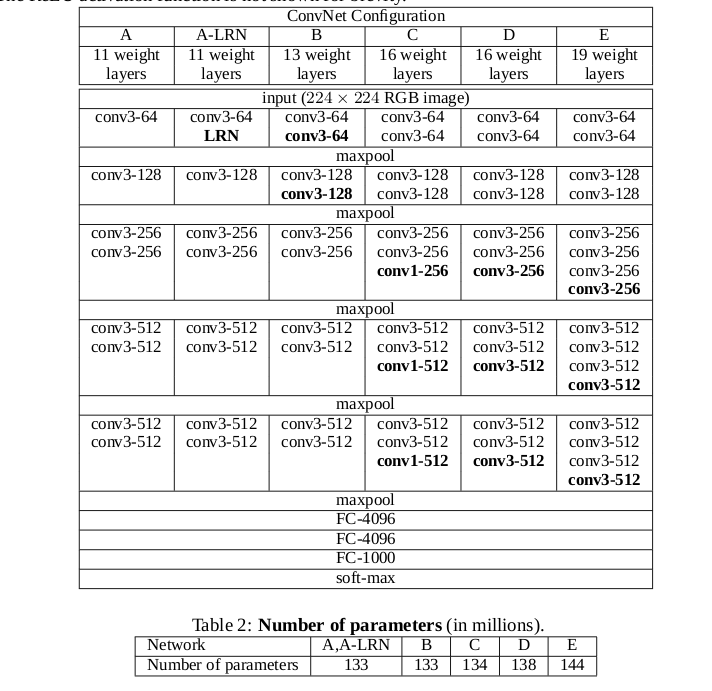
\includegraphics[width=.9\linewidth]{pics/vgg.png} \\

In spite of a large depth, the number of weights in our nets is not greater than the number of weights \\
in a more shallow net with larger conv. layer widths and receptive fields. \\
(That's one reason of using small kernel) \\


benefits of using three 3 x 3 conv. layer instead of a single 7 x 7 layer: \\
\begin{enumerate}
\item incorporate three non-linear rectification layers instead of a single one ==> make the decision function more discriminative \\
\item less parameters ==> imposing a regularisation on the 7 x 7 conv. filters, forcing them to have decomposition through the 3 x 3 filters \\
\end{enumerate}


The incorporation of 1 × 1 conv. layers is a way to increase the non-linearity \\
of the decision function without affecting the receptive fields of the conv. layers. \\

\subsection{classification framework}
\label{sec-2-4}

\subsubsection{training}
\label{sec-2-4-1}
The training is carried out by optimising the multinomial logistic regression objective \\
using mini-batch gradient descent (based on back-propagation (LeCun et al., 1989)) with momentum. \\

\begin{center}
\begin{tabular}{lr}
batch size & 256\\
momentum & 0.9\\
\end{tabular}
\end{center}

FC layers \\
first layer regularisation: weight decay (the $L_2$ penalty multiplier set to $5\cdot 10^{-4}$) \\
second layer regularisation: dropout (dropout ratio set to 0.5) \\


The learning rate was initially set to $10^{-2}$ , and then decreased by a factor of 10 when the validation set accuracy stopped improving. \\

The net converged after 74 epoches because of: (less epoches) \\
\begin{enumerate}
\item implicit regularisation imposed b greater depth and smaller convolution filter sizes \\
\item pre-initialisation of certain layers \\
\end{enumerate}


The initialisation of the network weights is important, since bad initialisation can stall learning \\
due to the instability of gradient in deep nets. ("Understanding the difficulty of training deep feedforward neural networks") \\

The author of this paper used pre-training emthod tu circumvent the initialisation of the network. \\
Although, the pre-training method is unnecessary for the initialisation, how is it done? \\


training set: \\
\begin{enumerate}
\item cropped from rescaled training images (one crop per image per SGD iteration) \\
\item random horizontal flipping \\
\item random RGB colour shift \\
\end{enumerate}

Training image size: \\
equal to or greater than 224 x 224. \\
If the image is greater than 224 x 224, a crop will be done. \\

isotropically-rescaled \emph{ai sou 'tro pi kerli} \\

scale jittering (one method of training set augmentation): \\
Each training image is individually rescaled by randomly sampling S from a certain range $[S_{min}, S_{max}]$ . \\
Crop S size input from sampled images. \\



\subsubsection{testing}
\label{sec-2-4-2}
\begin{enumerate}
\item rescale to a pre-defined smallest image side \\
\item network applied densely over the rescaled image \\
\item to obtain a fixed-size vector of class scores for the image, the class score is spatially averaged (sum-pooled) \\
\end{enumerate}

multi-crop evaluation vs dense evalution: \\



\subsection{classification experiments}
\label{sec-2-5}
Dataset: \\
\begin{center}
\begin{tabular}{ll}
training & 1.3M images\\
validation & 50K images\\
testing & 100K images\\
\end{tabular}
\end{center}


classification performance: \\
\begin{center}
\begin{tabular}{ll}
top-1 error & the portion of incorrectly classified images\\
top-5 error & the portion of images such that the ground-truth category is outside the top-5 predicted categories\\
\end{tabular}
\end{center}


\subsubsection{single scale evaluation}
\label{sec-2-5-1}

A deep net with small filters outperforms a shallow net with larger filters. \\
Training set augmentation by scale jittering is indeed helpful for capturing multi-scale image statistics \\

What is convolution boundary condition? \\

Emsembling improves the performance duo to complementarity of the models. \\

\subsection{Localisation}
\label{sec-2-6}

bounding box prediction: \\
SCR: single-class regression? \\
PCR: per-class regression? \\

logistic regression --> Euclidean loss \\

To come up with the final prediction: \\
greedy merging procedure \\
\begin{enumerate}
\item merge spatially close predictions (by averaging their coordinates) \\
\item rates them on the class scores \\
\end{enumerate}

localisation error in ILSVRC criterion: \\
$IoU = \frac{P\cap G}{P\cup G} < 0.5$  \\

Conclution: The preformance in localisation can be improved with very deep convolution nets. \\

\subsection{generalisation of very deep features}
\label{sec-2-7}
ConvNets, pre-trained on ILSVRC, generalise well on other, smaller, datasets, \\
where training large models from scratch is not feasible due to over-fitting. \\

How: \\
remove the lst fully-connected layer and use 4096-D activation of the penultimate layer as image features \\

aggregation of feature: \\
\begin{enumerate}
\item an image is rescaled \\
\item the network is densely applied \\
\item perform global average pooling on the resulting feature map (produces a 4096-D image descriptor) \\
\item the descriptor is averaged with the descriptor of a horizontally flipped image \\
\item extract feature over several scales \\
\item the resulting multi-scale features can be either stacked or pooled across scales \\
\end{enumerate}



20\% of training images were used as a validation set for hyper-parameter selection. \\
hyper-parameter: set by human being. (learning rate, tree depth) \\
parameter: learned from a algorithm. (matrix weight of CNN) \\


If the dataset contains multi-scale image, stacking and pooling of feature are almost same. \\
Otherwise, stacking allows a classifier to expolit scale-specific representations, and behaves better. \\



\section{visualizing and understanding convolutional networks}
\label{sec-3}
\subsection{intruduction}
\label{sec-3-1}
Without clear understanding of how and why they work, the development of better models \\
is reduced to trial-and-error. \\

To study the CNN: \\
\begin{enumerate}
\item visualizing with multi-layer deconvolutinal network \\
\item sensitivity analysis of the classifier output by occluding portions of the input images. \\
\end{enumerate}


\subsection{Approach}
\label{sec-3-2}
deconvnet: map features to pixels \\

switches: record the location of the local max in each pooling region. \\

In convnet, the max pooling operation is non-invertible, however we can obtain an approximate \\
inverse with \textbf{swithes} \\
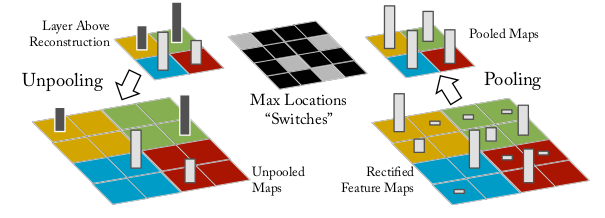
\includegraphics[width=.9\linewidth]{pics/switches.png} \\

As these switch settings are peculiar to a given input image, the reconstruction obtained from \\
a single activation thus resembles a small piece of the original input image, with structures \\
weighted according to their contribution toward to the feature activation. \\

deconvent: \\
\begin{enumerate}
\item unpooling with switches \\
\item rectification with relu (same with convnet) \\
\item filtering with transposed filter \\
\end{enumerate}


\subsection{Training Details}
\label{sec-3-3}
preprocess: \\
\begin{enumerate}
\item resize the smallest dimension to 256 \\
\item crop the center 256*256 region \\
\item substracting the per-pixel mean \\
\item use 10 different sub-corps of size 224*224 \\
\end{enumerate}

optimization: \\
SGD with mini-batch (128) \\

Renormalize each filter whose RMS(root mean square) value exceeds a fixed radius of $10^{-1}$ to this fixed radius \\
to avoid a few of filters dominate. \\

\subsection{Convnet Visualization}
\label{sec-3-4}
\subsubsection{Feature visualization}
\label{sec-3-4-1}
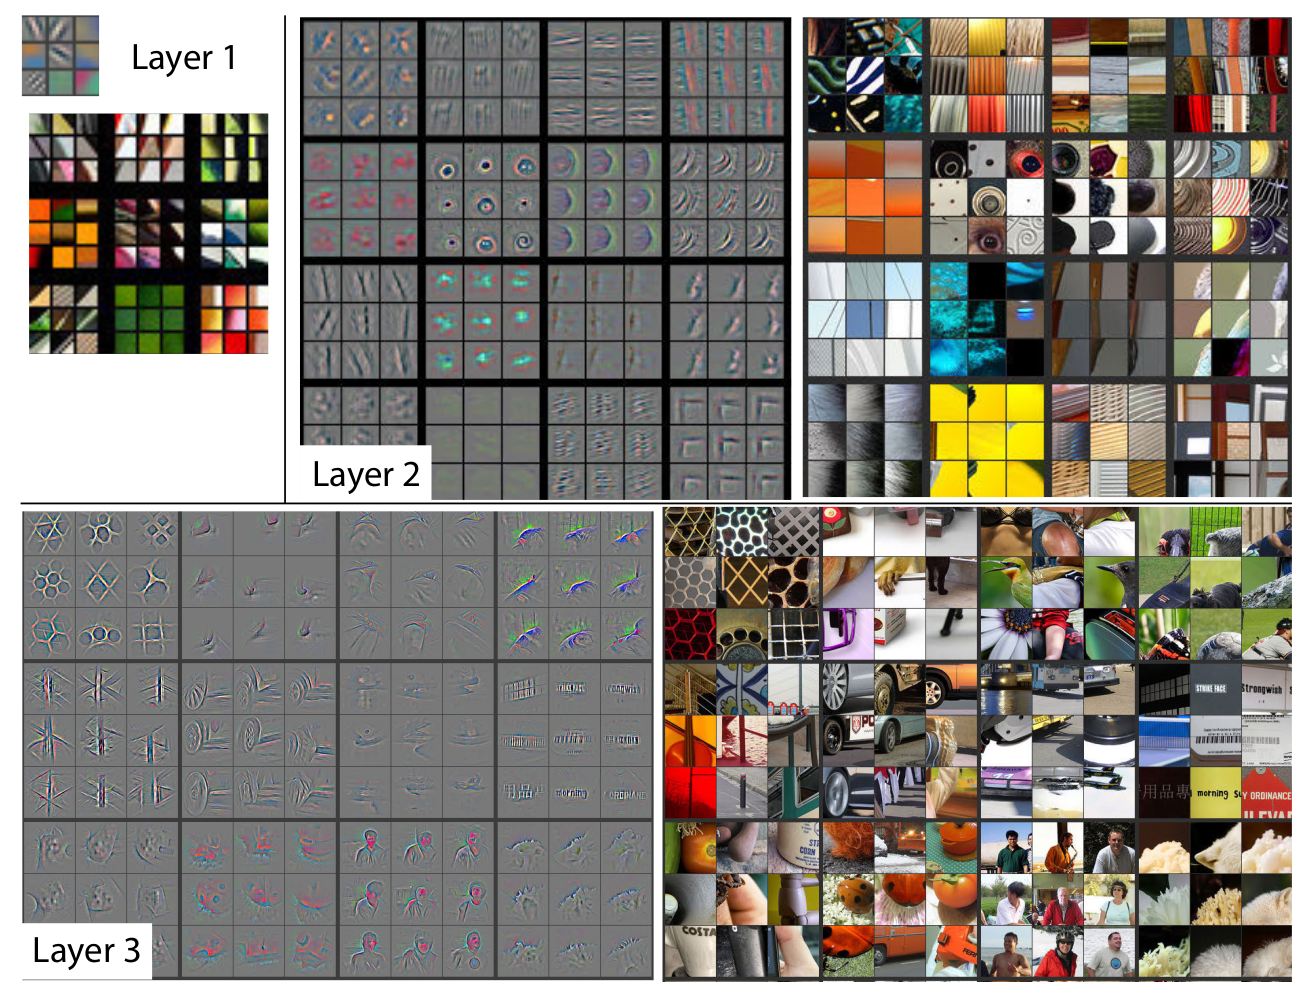
\includegraphics[width=.9\linewidth]{pics/cnn-feature-visualization.png} \\
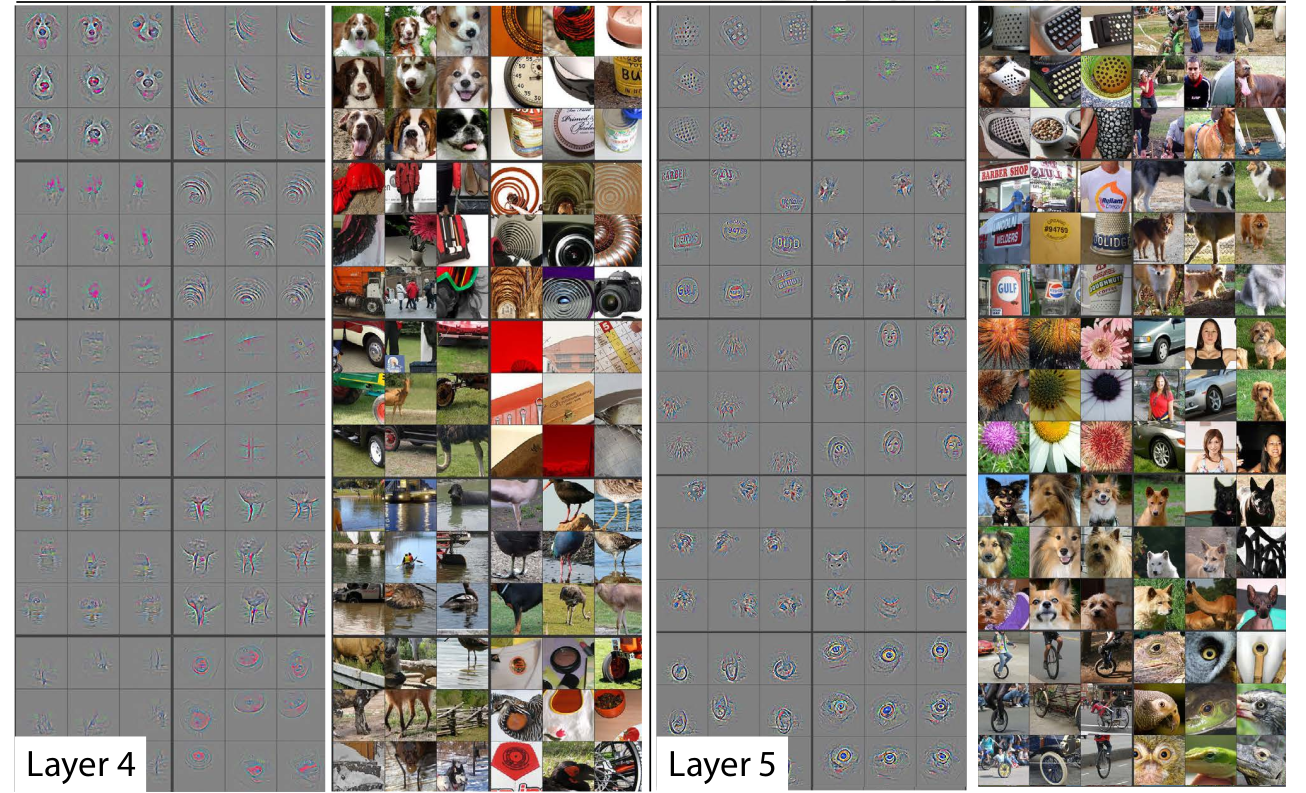
\includegraphics[width=.9\linewidth]{pics/cnn-feature-visualization2.png} \\
\begin{enumerate}
\item strong grouping within each feature map \\
\item greater invariance at higher layers \\
\item exaggeration of discriminative parts of the image \\
\end{enumerate}


\subsubsection{Feature Evolution during Training}
\label{sec-3-4-2}
The latter layer need more epoches to converge. \\


\subsubsection{Feature Invariance}
\label{sec-3-4-3}
For max pooling, the network output is stable to translations and scaling. \\
In general, the output is not invariant to rotation. \\



\subsubsection{Occlusion Sensitivity}
\label{sec-3-4-4}
method: occlude different parts of the image. \\

The model is localizing the objects as the probability of the correct class drops significantly \\
when the object is occluded. \\

This shows that the visualization genuinely corresponds to the image structure \\
that stimulates that feature map. \\


\subsubsection{Correspondence Analysis}
\label{sec-3-4-5}
method: masking out specified parts and random parts of a image. \\

At layer 5, the model does establish some degree of correspondence \\
by comparing Mean Feature Sign Change with masking out left eye, right eye, nose and random region. \\


\section{BIM Tracker: A model based visual tracking approach for indoor localisation using a 3D building model}
\label{sec-4}
localization with edges search and matching. \\
\section{BIM-PoseNet: Indoor camera localisation using a 3D indoor model and deep}
\label{sec-5}
result: indoor localization in real-time with an accuracy of approximately 2 meters. \\
\subsection{Introduction}
\label{sec-5-1}
objective: investigate whether pose estimation can be done by fine-tuning a pre-trained \\
           network using synthetic images derived from a 3D indoor model rather than geotagged images \\
\subsection{Background and related work}
\label{sec-5-2}
The visual localization approaches in the literature can be classified as: \\
\begin{description}
\item[{appearance-based}] image retrieval problem \\
\item[{pose eistimation-base}] directly estimate the 6-DOF pose of a \\
\begin{description}
\item[{matching point features with 3D point clouds}] requirement of point clouds (usually derived from SfM) \\
\item[{pose regression using RGB-D images}] fast and precise, but need RGB-D camera \\
\item[{pose regression using images only}] 
\end{description}
\end{description}

RGB-D: RGB + depth (distance between pixel and the sensors) \\

They fine-tuned a pre-trained network on image samples with ground-truth poses derived from the SfM methods. \\

They state: deep convolutional neural network trained for the task of classification preserve pose information \\
till the final layer by leveraging transfer learning, \\
despite being trained for a different task with a different dataset. \\

drawback (using ground-truth images): dependent on SfMmethods to estimate the ground truch camera poses, \\
required during fine-tuning the network. \\

synthetic images generated from 3D object models is used to eliminate the challenge of creating \\
manually labelled images (ground truth images) \\
\subsection{Methodology}
\label{sec-5-3}
current CNN network -> based on -> PoseNet(Kendall,2015) -> based on -> GoogLeNet(Szegedy,2015) \\

Thw weights are updated from a pre-trained network of GooLeNet that is trained on Places dataset(Zhou,2014) \\

\begin{equation}
p=[x,q]
\end{equation}
x is a vector representing; \\
q is a orientation representing; \\

\begin{equation}
\mathrm{loss}(I)=||\hat{x}-x||_2+\beta \left |\left | \hat{q}-\frac{q}{||q||} \right | \right |_2
\end{equation}

$\beta$ is a hyperparameter balancing the error of location and orientation. \\



The author of (Peng,2015) show that features derived from DCNNs are invariant to color, texture, pose and context. \\
In other words, if a network is invariant to an object's texture, \\
then it will have similar activations of neurons for the object with or without texture. \\
The network hallucinates the right texture when given a texutre-less object's shape. \\
(? don't understand) \\

Whether different model renderings and processing the real images to make them similar \\
to the synthetic images will increase the pose estimation accuracy. \\

To test this, we transform the synthetic and real images in a common feature space of edge gradient magnitude (gradmag) images. \\
(Converting images to edge gradmag comes at the cost of loss of information such as \\
colour and texture, but on the other hand, the main geometrical features of the images are preserved. ) \\
\subsection{experiments and result}
\label{sec-5-4}
\begin{enumerate}
\item experiment 1: creating a baseline accuracy using real images \\
\item experiment 2: fine-tuning with synthetic image dataset and test \\
\item experiment 3: explore accuracy with detail \\
\end{enumerate}

\begin{center}
\begin{tabular}{ll}
 & Caffe library on Linux\\
loss optimization & Adagrad gradient descent optimization algorithm\\
learing rate & $10^{-3}$.\\
 & NVIDIA GTX980M\\
batch size & 40\\
resize to resolution & 320*240\\
crop & 224*224\\
 & \\
\end{tabular}
\end{center}
\subsubsection{dataset}
\label{sec-5-4-1}
\begin{enumerate}
\item synthetic image dataset
\label{sec-5-4-1-1}
The BIM contains the main building elements including walls, floors, ceilings, doors, ceiling tube-lights, \\
and stairs, but not details such as material, fabrication, assembly and installation information \\

The height of the trajectory was kept in the range of $1.5 - 1.8$ meters from the floor. \\

we have rendered images along the trajectory at 0.05 meters interval and $\pm 10$ tilt. \\
\item real image dataset
\label{sec-5-4-1-2}
A total number of 1000 images of 640x480 pixels resolution were acquired at a constant 30 frames per second. \\
\end{enumerate}
\subsubsection{baseline performance using real images}
\label{sec-5-4-2}
The value of $\beta$ lies in the range of 120 to 750. (beta seleted) \\

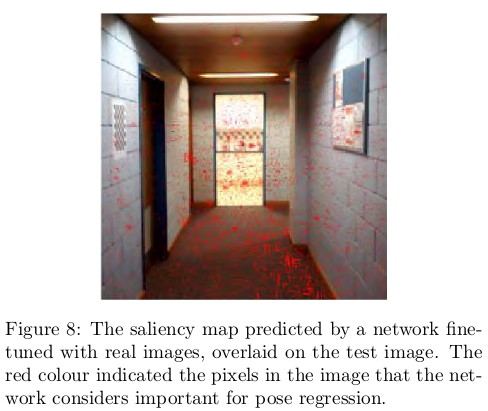
\includegraphics[width=.9\linewidth]{pics/saliency-map.png} \\

\subsubsection{fine-tuning with synthetic images}
\label{sec-5-4-3}
The author showed that: different parts of a image make a difference in importance. \\

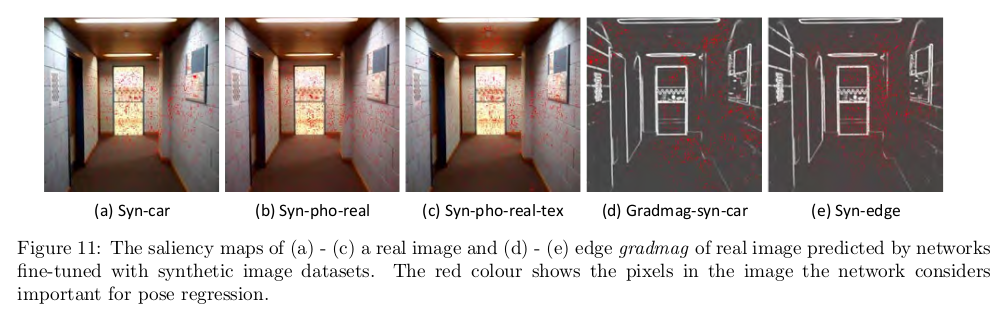
\includegraphics[width=.9\linewidth]{pics/dif-importance.png} \\


elements to case error: \\
\begin{enumerate}
\item photo blur \\
\item external elements (like poster) \\
\item structral difference \\
\end{enumerate}

Lighting of the scene plays a vital role in the appearance of the scene. \\

The high errors might be a result of the learnt features for each network, \\
which might not be suitable for pose regression with real images. \\
This fact is reflected in the saliency maps of the real images as predicted by the fine-tuned networks. \\

\subsection{effects of level-of-detail of 3D models}
\label{sec-5-5}
\section{Learning to Compare Image Patches via Convolutional Neural Networks}
\label{sec-6}
show how to learn directly from image data a general similarity function for comparing image patches. \\

Requirement: large datasets that contain patch correspondences between images. \\
This is not suitable from indoor localization, becuase this is no such large \\
dataset of camera pictures. \\
\section{Structure Extraction from Texture via Relative Total Variation}
\label{sec-7}
a picture = meaningful structures + textured surfaces (commonly) \\

inherent variation and relative total variation to distinguish them \\

In psychology: \\
the overall structural features are the primary data \\
of human perception, not the individual details \\
\section{Cross-Domain 3D Model Retrieval via Visual Domain Adaptation}
\label{sec-8}
\section{Cross-domain Image Retrieval with a Dual Attribute-aware Ranking Network}
\label{sec-9}
DARN: Dual Attribute-aware Randing Network \\

retrieval feature learing. \\

two sub-networks, whose retrieval feature representations are driven by semantic attribute learning. \\

attribute-guided learning is a key factor for retrieval accuracy improvement. \\

\subsection{Related Work}
\label{sec-9-1}
\begin{enumerate}
\item Fashion Dataset \\
\item Visual Analysis of Clothing with Fashion Datasetn \\
\item Visual Attibutes \\
\item Deep Learning (explicitly use attribute prediction as a regularizer in deep network) \\
\end{enumerate}

Attributes are usually referred as semantic properties of objects or scenes that are shared across categories. \\

Richer supervision conveying annotator /'an nou tei ter/ rationales based on visual attributes, can be considered as a form of privileged information. \\
Cross-domain image retrieval can benefit from feature learning that simultaneously optimizes a loss function that takes into account visual similarity and attribute classification. \\

A poselet describes a particular part of the human pose under a given viewpoint. \\

\subsection{Data Collection}
\label{sec-9-2}
% Emacs 25.2.2 (Org mode 8.2.10)
\end{document}
